\documentclass[conference]{IEEEtran}
\IEEEoverridecommandlockouts
\usepackage{cite}
\usepackage{url}
\usepackage{amsmath,amssymb,amsfonts}
\usepackage{graphicx}
\usepackage{textcomp}
\usepackage{booktabs}
\usepackage{array}
\usepackage{tikz}
\usetikzlibrary{arrows.meta,positioning,fit,backgrounds,calc}

\renewcommand{\arraystretch}{1.15}
\setlength{\tabcolsep}{3pt}

\begin{document}

\title{Impact of Deep Compression on Deployed, Phase-Specific Accuracy in TCN for Real-Time Gait Detection}

\author{\IEEEauthorblockN{Anonymous Author(s)}
\IEEEauthorblockA{Affiliation withheld for double-anonymous review}}

\maketitle

\begin{abstract}
Wearable-based gait phase detection is a critical enabler for rehabilitation monitoring, fall-risk
assessment, and assistive robotics, yet deploying deep learning models on resource-constrained
microcontrollers remains challenging. This study evaluates INT8 post-training quantization and
structured channel pruning for a Standard TCN classifying gait phases (LR, LS, PSw, Sw) from
shank-mounted IMU data (NONAN GaitPrint), on the ESP32-C3, under subject-wise 5-fold
cross-validation ($K{=}5$, three seeds; $N{=}15$ runs per config).
TCN achieved the highest mean macro F1 among compared architectures ($90.87\%\pm1.47\%$),
significantly outperforming CNN1D ($+0.53$~pp, $p{=}0.004$) while statistically tying Transformer
($p{=}0.80$) and LSTM+GRU ($p{=}0.17$). A PyTorch weight-only quantize-dequantize (QDQ) proxy
suggests INT8 is lossless ($90.88\%\pm1.47\%$ vs.\ FP32; $p{=}0.30$); evaluating the
\emph{actual deployed} full-integer TFLite model on the complete test set confirms this proxy is
reasonable but not exact: plain INT8 costs a further $0.72\pm0.60$~pp ($p{=}1.8\times10^{-4}$),
while combined INT8+Prune50 costs $3.56\pm2.10$~pp---roughly double its proxy's estimate
($-$1.54~pp)---indicating the proxy--deployment gap widens as compression techniques stack.
Structured pruning, which involves no quantization and carries no such gap, reduces macro F1 by
1.47~pp at 50\% retention (5-epoch fine-tune; $p{<}0.001$), recoverable to $-$0.53~pp with 50
epochs. PSw and LR (transition phases) remain the most compression-sensitive under both pruning
and quantization, though the real INT8 effect is modest (LR $-$1.6~pp, PSw $-$0.8~pp). Since
PSw/LR each span only ${\sim}50$--$100$~ms of the gait cycle, we adopt a clinically motivated
100~ms real-time budget rather than the coarser 500~ms offline-evaluation window: only
INT8+Prune50 (75.7~ms) meets it on ESP32-C3, while INT8 (279.8~ms), Prune50 (253~ms), Prune75
(510.8~ms), and FP32 (856~ms) do not---the smallest, most quantization-dependent config is also
the only one fast enough to resolve transitions in real time.
\end{abstract}

\begin{IEEEkeywords}
TCN, deep compression, post-training quantization, TFLite, deployment validation, pruning, gait
phase detection, ESP32-C3, edge AI, wearable sensors
\end{IEEEkeywords}

\section{Introduction}

Accurate detection of gait phases---such as loading response, mid-stance, pre-swing, and
swing---is fundamental to applications in clinical rehabilitation, fall prevention, prosthetic
control, and sports biomechanics. Recent advances in deep learning, particularly recurrent and
convolutional architectures, have substantially improved gait phase classification accuracy using
wearable inertial measurement unit (IMU) sensors. However, these models are typically designed and
validated on desktop or server-class hardware, and their large parameter counts and floating-point
computations make them impractical for direct deployment on low-power, low-memory microcontrollers
used in real-world wearable devices.

Temporal Convolutional Networks (TCNs), which leverage dilated convolutions to capture long-range
temporal dependencies with fewer parameters than recurrent architectures, offer a promising middle
ground between accuracy and efficiency and can be further compressed via quantization and pruning
to meet the strict memory and latency budgets of microcontroller-class hardware such as the ESP32-C3.
While prior work has explored model compression broadly for time-series classification, little
attention has been paid to how compression affects accuracy unevenly across gait phases. Transition
phases such as Loading Response (LR) and Pre-Swing (PSw) are inherently more ambiguous due to
overlapping biomechanical signal characteristics, and we hypothesize these are more vulnerable to
information loss from aggressive quantization and pruning than steady-state phases such as Swing (Sw).

This study addresses this gap by:
\begin{enumerate}
  \item Selecting and training a Standard TCN backbone for gait phase classification using shank
        IMU data from NONAN GaitPrint, with matched-capacity FP32 baselines for context;
  \item Systematically applying INT8 quantization and structured pruning, quantifying their impact
        on phase-specific accuracy and F1-score rather than overall accuracy alone;
  \item Deploying the compressed models on ESP32-C3 hardware and measuring on-device latency and
        SRAM headroom against a clinically motivated real-time budget;
  \item Validating whether a common PyTorch-side weight-only quantization proxy predicts the
        \emph{actual deployed} full-integer TFLite model's accuracy, at the same statistical rigor
        ($N{=}15$) as the rest of this paper, and showing this proxy--deployment gap widens as
        compression techniques are combined.
\end{enumerate}

\section{Literature Review}
\label{sec:litreview}

\subsection{Gait Phase Detection Using Wearable IMU Sensors}

Gait phase detection using body-worn IMU sensors has been extensively studied, with shank- and
foot-mounted sensors commonly used due to their high sensitivity to phase transitions. Classical
approaches (threshold-based, hidden Markov models) have largely been superseded by deep learning
methods---1D CNNs, LSTM, hybrid LSTM+GRU, and, more recently, Transformer encoders---which learn
temporal dependencies directly from raw or lightly processed signals. Using the same NONAN
GaitPrint dataset and shank-mounted six-axis IMU configuration, Choi and Choi~\cite{ref1} directly
compared a 1D CNN, a hybrid LSTM+GRU model, and a Transformer for four-class gait phase
classification, reporting comparable performance (macro F1 ${\approx}91$--93\%) with the
Transformer attaining the highest score. The present study replicates those three architectures,
plus a standard TCN, as FP32 baselines under an identical protocol (Section~\ref{sec:method}), but
targets a distinct research question left open by prior work: how INT8 quantization and structured
pruning affect \emph{phase-specific} accuracy, and how the resulting models perform when deployed
on microcontroller-class hardware.

\subsection{Temporal Convolutional Networks (TCNs) for Time-Series Classification}

TCNs use causal, dilated convolutions to achieve large receptive fields with a fraction of the
parameters required by recurrent architectures, while supporting parallelized
computation~\cite{ref2}, making them attractive for edge deployment where both parameter count and
latency are critical. All architectures here share a common hidden width (32 channels) and 0.5~s
causal windows, yielding 10--26K-parameter models sized for ESP32-C3 rather than server-scale
capacity.

\subsection{Model Compression Techniques: Quantization and Pruning}

Post-training quantization reduces numerical precision (e.g., FP32$\to$INT8), reducing model size
and enabling faster, more energy-efficient inference on integer-optimized hardware~\cite{ref3}.
Structured pruning removes entire channels or filters, yielding actual speedups on commodity
hardware (unlike unstructured pruning, which needs sparse-matrix support)~\cite{ref4}. Both are
widely studied for image and audio models, but their differential effect across distinct temporal
phases of a periodic signal---such as gait phases---and the gap between simulated and deployed
quantization accuracy, remain comparatively underexplored; this study addresses both directly.

\subsection{Edge AI Deployment on Microcontrollers (ESP32-C3)}

TensorFlow Lite Micro (TFLM) enables compact neural networks to run directly on microcontroller
hardware with kilobyte-scale memory budgets~\cite{ref5}. The ESP32-C3 is a single-core RISC-V
microcontroller (160~MHz, ${\approx}400$~KB SRAM~\cite{ref6}), a low-cost TinyML target that lacks
the vector acceleration of higher-end Espressif parts, motivating its use here to stress-test
compressed models under real hardware constraints.

\section{Methodology}
\label{sec:method}

\subsection{Dataset and Preprocessing}

\begin{itemize}
  \item \textbf{Dataset:} NONAN GaitPrint~\cite{ref7}, using shank-mounted IMU channels
        (accelerometer and gyroscope axes).
  \item \textbf{Sampling rate:} Original 200~Hz signal downsampled to 100~Hz for all reported
        experiments, balancing temporal resolution against on-device resource constraints.
  \item \textbf{Labeling:} Gait cycle phases labeled as Loading Response (LR), Loading Stance (LS),
        Pre-Swing (PSw), and Swing (Sw).
  \item \textbf{Data split:} Subject-wise stratified 5-fold CV ($K{=}5$) with three seeds;
        validation subjects rotate per fold (re-sampled from the non-test pool) to avoid
        repeated early-stopping bias; no subject leakage across train/val/test.
  \item \textbf{Normalization:} Per-channel z-score normalization computed on the training set only.
  \item \textbf{Windowing:} Causal 0.5~s windows with train stride~5 and validation/test stride~1
        (test windows overlap $\approx$98\%; per-subject blocked macro F1 reported alongside
        window-level metrics).
  \item \textbf{Training:} Adam optimizer ($\mathrm{lr}=10^{-3}$), batch size 512, up to 50 epochs;
        best checkpoint selected by validation macro F1.
  \item \textbf{Fair comparison design:} All architectures use hidden width 32, four-class output,
        identical windowing/optimization/CV splits, and capped capacity (${\sim}10$--26K params,
        ${\sim}40$--100~KB FP32) rather than maximizing accuracy with large networks.
  \item \textbf{Compression fine-tuning:} Pruning uses \emph{training subjects only} (fixed epoch
        budget, no validation access) to avoid double-dipping on the FP32 checkpoint-selection
        validation set; runtime assertions verify zero subject overlap for every fold.
  \item \textbf{Evaluation:} Table~\ref{tab:baseline} reports mean$\,\pm$\,std macro F1 over
        $K{=}5$ folds$\times$3 seeds ($N{=}15$ runs) with paired Wilcoxon tests; compression results
        (Table~\ref{tab:kfold-compression}), the fine-tune ablation
        (Table~\ref{tab:finetune-ablation}), and real deployed TFLite accuracy for INT8/INT8+Prune50
        (Table~\ref{tab:int8-real}) use the same protocol. Figs.~\ref{fig:pareto}
        and~\ref{fig:phase-degradation} illustrate one fold/seed (0/42); Table~\ref{tab:esp32}
        reports ESP32-C3 latency for five deployable configs from that checkpoint.
\end{itemize}

Phase support is highly imbalanced (LS and Sw together account for
$(1{,}274{,}499+1{,}016{,}857)/2{,}583{,}680 \approx 88.7\%$ of test windows, vs.\ only
$11.3\%$ for the transition phases LR and PSw combined). To prevent the majority phases from
dominating optimization, all models---including the four FP32 baselines and every compression
fine-tuning stage---are trained with a class-balanced weighted cross-entropy loss:
\begin{equation}
  \mathcal{L} = -\sum_{c=1}^{4} \alpha_c \, y_c \log \hat{y}_c,
  \qquad
  \alpha_c = \frac{N}{4 \cdot N_c},
  \label{eq:loss}
\end{equation}
where $N$ is the number of training windows, $N_c$ is the number of windows labeled with phase
$c$, $y_c$ is the one-hot ground-truth indicator, and $\hat{y}_c$ is the softmax output
probability for phase $c$. This directly motivates reporting \emph{macro}, rather than
micro-averaged, metrics throughout this paper.

\subsection{TCN Architecture}

We adopt a Standard TCN~\cite{ref2} as the deployment backbone. The model consists of four dilated
causal convolutional blocks (dilation rates 1, 2, 4, and 8) with residual connections, batch
normalization, and a lightweight classification head (global average pooling followed by a dense
softmax layer over the four phase classes). Each block computes a dilated causal convolution
(kernel size $k{=}3$, dilation $d$, ReLU) so that each output depends only on present and past inputs.
Stacking four such blocks yields a receptive field of 31 samples (0.31~s at 100~Hz), comfortably
within the 0.5~s (50-sample) input window while keeping the parameter count near 11K. The model
consumes causal 0.5-second windows (50 samples at 100~Hz). Channel width is deliberately kept narrow
(32 hidden channels) to retain a microcontroller-deployable footprint (${\sim}45$~KB FP32).
Fig.~\ref{fig:architecture} illustrates the overall data flow and the internal structure of each
causal convolutional block.

\begin{figure}[!t]
  \centering
  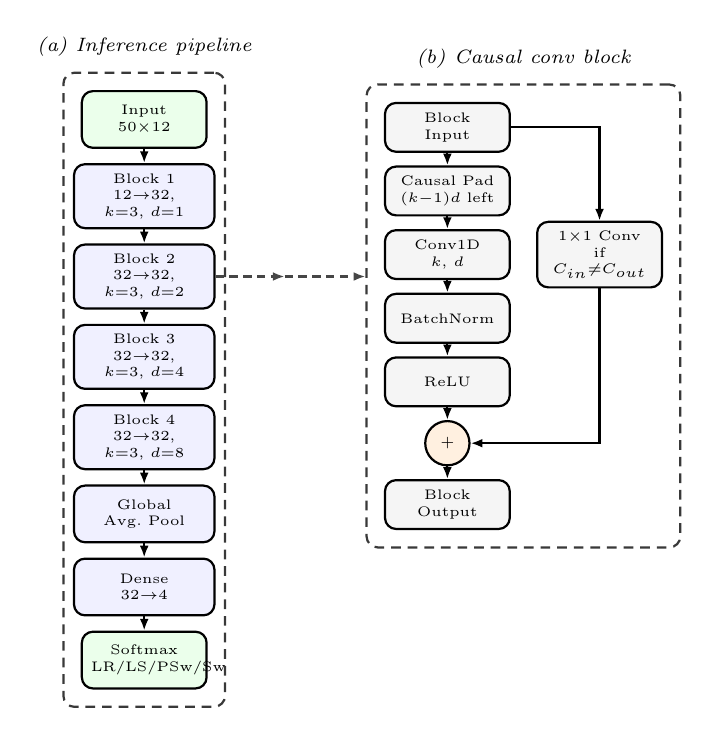
\begin{tikzpicture}[
      block/.style={rectangle, draw, thick, fill=blue!6, rounded corners,
        text width=1.55cm, minimum height=0.72cm, align=center, font=\tiny},
      io/.style={rectangle, draw, thick, fill=green!8, rounded corners,
        text width=1.35cm, minimum height=0.72cm, align=center, font=\tiny},
      sblock/.style={rectangle, draw, thick, fill=gray!8, rounded corners,
        text width=1.35cm, minimum height=0.62cm, align=center, font=\tiny},
      sum/.style={circle, draw, thick, fill=orange!12, minimum size=0.42cm, font=\tiny},
      arr/.style={thick, -{Latex[length=1.5mm]}},
      darr/.style={thick, dashed, draw=gray!55!black, dash pattern=on 3pt off 2pt,
        -{Latex[length=1.5mm]}},
      panel/.style={draw, dashed, draw=gray!45!black, dash pattern=on 3.5pt off 2.5pt,
        thick, inner sep=0.22cm, rounded corners}
    ]

    % --- (a) Vertical inference pipeline ---
    \node[io] (input) {Input\\$50{\times}12$};
    \node[block, below=0.18cm of input] (b1) {Block 1\\$12{\to}32$, $k{=}3$, $d{=}1$};
    \node[block, below=0.18cm of b1] (b2) {Block 2\\$32{\to}32$, $k{=}3$, $d{=}2$};
    \node[block, below=0.18cm of b2] (b3) {Block 3\\$32{\to}32$, $k{=}3$, $d{=}4$};
    \node[block, below=0.18cm of b3] (b4) {Block 4\\$32{\to}32$, $k{=}3$, $d{=}8$};
    \node[block, below=0.18cm of b4] (gap) {Global\\Avg.\ Pool};
    \node[block, below=0.18cm of gap] (fc) {Dense\\$32{\to}4$};
    \node[io, below=0.18cm of fc] (out) {Softmax\\LR/LS/PSw/Sw};

    \draw[arr] (input) -- (b1);
    \draw[arr] (b1) -- (b2);
    \draw[arr] (b2) -- (b3);
    \draw[arr] (b3) -- (b4);
    \draw[arr] (b4) -- (gap);
    \draw[arr] (gap) -- (fc);
    \draw[arr] (fc) -- (out);

    \node[panel, fit=(input)(out),
      label={[font=\scriptsize\itshape, yshift=2pt]above:(a) Inference pipeline}] (pipebox) {};

    % --- (b) Causal conv block detail (right panel) ---
    \begin{scope}[xshift=3.85cm, yshift=-0.1cm]
      \node[sblock] (bin) {Block\\Input};
      \node[sblock, below=0.16cm of bin] (pad) {Causal Pad\\$(k{-}1)d$ left};
      \node[sblock, below=0.16cm of pad] (conv) {Conv1D\\$k$, $d$};
      \node[sblock, below=0.16cm of conv] (bn) {BatchNorm};
      \node[sblock, below=0.16cm of bn] (relu) {ReLU};
      \node[sum, below=0.16cm of relu] (add) {$+$};
      \node[sblock, below=0.16cm of add] (bout) {Block\\Output};
      \node[sblock, right=0.32cm of conv] (resid) {$1{\times}1$ Conv\\if $C_{in}{\neq}C_{out}$};

      \draw[arr] (bin) -- (pad);
      \draw[arr] (pad) -- (conv);
      \draw[arr] (conv) -- (bn);
      \draw[arr] (bn) -- (relu);
      \draw[arr] (relu) -- (add);
      \draw[arr] (add) -- (bout);
      \draw[arr] (bin.east) -| (resid.north);
      \draw[arr] (resid.south) |- (add.east);

      \node[panel, fit=(bin)(bout)(resid),
        label={[font=\scriptsize\itshape, yshift=2pt]above:(b) Causal conv block}] (detailbox) {};
    \end{scope}

    \coordinate (linkmid) at ($(pipebox.east)!0.42!(detailbox.west)$);
    \draw[darr] (b2.east) -- ($(linkmid |- b2.east)+(0,0)$);
    \draw[darr] (linkmid |- b2.east) -- (detailbox.west |- b2.east);
  \end{tikzpicture}
  \caption{Standard TCN architecture: (a) end-to-end pipeline from a $50{\times}12$ causal window to
  a 4-class softmax, and (b) internal structure of each causal convolutional block (left-padding,
  dilated Conv1D, batch norm, ReLU, and residual connection).}
  \label{fig:architecture}
\end{figure}

\subsection{Baseline Architectures for Context}

For context, three FP32 baselines (CNN1D, LSTM+GRU, Transformer) were retrained under the same
hidden width, windowing, and cross-validation protocol (Table~\ref{tab:baseline}).

\subsection{Deep Compression Protocol}

\textbf{Post-training quantization (INT8).} We apply symmetric 8-bit quantization separately to
each convolutional and fully connected weight layer. For every layer, a single scale is set from
that layer's largest absolute weight; each weight is rounded to the nearest integer in
$[-127,127]$, then mapped back to floating point for inference. This quantize--dequantize (QDQ)
proxy is used for PyTorch-side test-set evaluation (Section~\ref{sec:results}). For ESP32
deployment, models are exported as full-integer TensorFlow Lite graphs (100 calibration windows
from training subjects). Real deployed accuracy is measured by running the exact exported artifact
through a TFLite interpreter with a saturating int8 cast ($[-127,127]$), matching the firmware.

\textbf{Structured channel pruning.} The TCN stem uses 32 hidden channels. Channels are ranked by summed absolute weight magnitude across all stem
convolutional blocks; the top-$k$ channels are retained and removed elsewhere in the stem and
classification head. The pruned model is fine-tuned on \emph{training subjects only} (Adam,
learning rate $10^{-4}$, class-balanced loss) before re-evaluation. Primary k-fold configs sweep
25\%, 50\%, and 75\% channel retention (Prune25/50/75; Prune25 \emph{retains} 25\% and is thus
the most aggressive setting, Prune75 the mildest) with a default 5-epoch fine-tune budget, reported
in Table~\ref{tab:kfold-compression} at $N{=}15$; Table~\ref{tab:finetune-ablation} separately
ablates the fine-tune epoch budget at a fixed 50\% retention.

\textbf{Extended compression grid (k-fold).} Beyond FP32/INT8 and Prune25/50/75, combined
INT8+Prune50 populates the Pareto front (Fig.~\ref{fig:pareto}). INT4 is excluded because
full-integer INT4 TFLite is not supported on the ESP32-C3 deployment target.
Fine-tune schedule ablation on Prune50 (5/15/50 epochs) isolates whether accuracy loss under
pruning reflects insufficient recovery training rather than an inherent pruning limit
(Table~\ref{tab:finetune-ablation}).

Compression variants comprise INT8 post-training quantization (PyTorch QDQ proxy for test metrics;
full-integer TFLite PTQ for ESP32), structured 25/50/75\% channel pruning with train-only
fine-tuning, and combined INT8+Prune50.

\subsection{Hardware Deployment (ESP32-C3)}

After PyTorch compression evaluation, selected models are converted to TensorFlow Lite (.tflite)
format and deployed via TensorFlow Lite Micro on an ESP32-C3 development board (160~MHz, Arduino
IDE, Chirale\_TensorFlowLite). On-device inference latency is measured per 0.5-second input window
over 1000 timed trials (20 warmup invocations), alongside minimum free heap during benchmarking and
a fixed 120~KB tensor arena.

\subsection{Evaluation Metrics}

Macro F1 is the unweighted mean of the four per-phase F1 scores. Unlike accuracy or a
support-weighted average, this gives Loading Response (LR) and Pre-Swing (PSw) equal weight to the
majority phases despite their $\sim\!6\%$ and $\sim\!5\%$ test-set support, respectively.

\begin{itemize}
  \item Phase-specific F1 and accuracy for LR, LS, PSw, and Sw.
  \item Pareto analysis: macro F1 vs.\ model size (KB) per compression config.
  \item On-device latency (ms) and minimum free heap (KB) on ESP32-C3.
\end{itemize}

\section{Results}
\label{sec:results}

\subsection{Baseline Comparison and Model Complexity}

Table~\ref{tab:baseline} compares TCN against three FP32 baselines under the primary
$K{=}5\times3$ protocol (mean$\,\pm$\,std over 15 runs). Macro F1 scores cluster tightly
(90.34--90.87\%); TCN attains the highest mean macro F1 ($90.87\%\pm1.47\%$). Paired Wilcoxon
tests on matched fold$\times$seed pairs show TCN statistically equivalent to Transformer
($\Delta{=}{+}0.04$~pp, $p{=}0.80$) and LSTM+GRU ($+0.28$~pp, $p{=}0.17$), but significantly
higher than CNN1D ($+0.53$~pp, $p{=}0.004$).

\begin{table}[!t]
  \centering
  \caption{Baseline FP32 Comparison ($K{=}5\times3$ Seeds)}
  \label{tab:baseline}
  \scriptsize
  \setlength{\tabcolsep}{2.8pt}
  \renewcommand{\arraystretch}{1.1}
  \begin{tabular}{@{} l r r c *{4}{c} @{}}
    \toprule
    \textbf{Model} & \textbf{Params} & \textbf{KB} & \textbf{Macro F1 (\%)} &
    \multicolumn{4}{c}{\textbf{Phase F1 (\%)}} \\
    \cmidrule(lr){5-8}
    & & & & \textbf{LR} & \textbf{LS} & \textbf{PSw} & \textbf{Sw} \\
    \midrule
    TCN &
      11{,}560 & 45.2 & \textbf{90.87\,$\pm$\,1.47} &
      \textbf{85.81} & \textbf{97.78} & 82.72 & 97.18 \\
    Transformer &
      25{,}956 & 101.4 & 90.83\,$\pm$\,0.99 &
      85.37 & 97.73 & \textbf{82.95} & \textbf{97.27} \\
    LSTM+GRU &
      12{,}356 & 48.3 & 90.59\,$\pm$\,1.19 &
      84.95 & 97.70 & 82.52 & 97.22 \\
    CNN1D &
      10{,}727 & 41.9 & 90.34\,$\pm$\,1.21 &
      84.32 & 97.52 & 82.54 & 97.00 \\
    \bottomrule
  \end{tabular}

  \vspace{0.45em}
  {\scriptsize Mean\,$\pm$\,std macro F1 ($N{=}15$); phase F1 reported as means. Hidden width 32 for all models.}
\end{table}

\subsection{TCN Compression Under K-Fold Cross-Validation}

Table~\ref{tab:kfold-compression} reports the primary compression results aggregated over
$N{=}15$ matched fold$\times$seed pairs, with paired Wilcoxon signed-rank tests against the FP32
reference (same checkpoints, no retraining).

% Auto-generated by analysis/export_kfold_compression_tex.py
% Re-run after: python analysis/aggregate_runs.py && python analysis/export_kfold_compression_tex.py
\begin{table}[!t]
  \centering
  \caption{TCN K-Fold Compression (Macro F1 \%, Mean\,$\pm\,$Std; $N{=}15$ per config)}
  \label{tab:kfold-compression}
  \scriptsize
  \setlength{\tabcolsep}{4pt}
  \renewcommand{\arraystretch}{1.08}
  \begin{tabular}{@{} l c @{\hspace{8pt}} c @{\hspace{4pt}} c @{}}
    \toprule
    \textbf{Config} & \textbf{Macro F1} & \textbf{PSw F1} & \textbf{Wilcoxon $p$ vs.\ FP32} \\
    \midrule
    FP32 & 90.87\,$\pm$\,1.47 & 82.72\,$\pm$\,2.54 & --- \\
    INT8 & 90.88\,$\pm$\,1.47 & 82.75\,$\pm$\,2.54 & 0.303 \\
    Prune25 & 87.62\,$\pm$\,1.45 & 78.97\,$\pm$\,1.28 & 6.10e-05 \\
    Prune50 & 89.40\,$\pm$\,1.43 & 81.13\,$\pm$\,1.97 & 6.10e-05 \\
    Prune75 & 90.17\,$\pm$\,1.30 & 81.90\,$\pm$\,2.18 & 6.10e-05 \\
    INT8+Prune50 & 89.33\,$\pm$\,1.36 & 80.93\,$\pm$\,2.00 & 1.22e-04 \\
    \bottomrule
  \end{tabular}

  \vspace{0.5em}
  {\scriptsize Paired Wilcoxon signed-rank tests on matched fold$\times$seed pairs ($N{=}15$) vs.\ FP32. All configs complete (120/120 jobs). $p{=}6.10\mathrm{e}{-05}$ is the $N{=}15$ Wilcoxon floor (see Limitations). Config names denote \% channels retained; Prune25 is most aggressive, Prune75 mildest.}
\end{table}


\textbf{The PyTorch QDQ proxy is a reasonable, but imperfect, stand-in for deployed INT8 accuracy.}
INT8 attains $90.88\%\pm1.47\%$ macro F1 ($+0.01$~pp vs.\ FP32; Wilcoxon $p{=}0.30$) with an
estimated payload of ${\sim}13.0$~KB (${\sim}3.4{\times}$ smaller than FP32) under the PyTorch
weight-only quantize-dequantize (QDQ) proxy used throughout Table~\ref{tab:kfold-compression}.
This proxy quantizes only weights; it does not model activation quantization noise. We therefore
evaluated the \emph{actual deployed} full-integer TFLite artifacts (Section~\ref{sec:esp32-results})
against the complete stride-1 test set (not a subsample) using the TFLite interpreter with a
saturating int8 cast matching the ESP32-C3 firmware, across the same primary protocol as the rest
of this paper ($N{=}15$: 5 folds $\times$ 3 seeds; Table~\ref{tab:int8-real}).

% Hand-authored from analysis/tflite_real_accuracy_summary.json (N=15: 5 folds x 3 seeds)
% Corrected 2026-07-24: earlier draft had an int8 cast overflow bug (no saturation) in the
% host-side evaluation harness, not present in the ESP32-C3 firmware; numbers below use a
% saturating cast matching the deployed firmware's quantization behavior.
\begin{table}[!t]
  \centering
  \caption{Real Deployed TFLite vs.\ PyTorch Accuracy (Macro F1 \%, TCN, $N{=}15$)}
  \label{tab:int8-real}
  \scriptsize
  \setlength{\tabcolsep}{3.5pt}
  \renewcommand{\arraystretch}{1.08}
  \begin{tabular}{@{} l c c c c @{}}
    \toprule
    \textbf{Config} & \textbf{Real TFLite} & \textbf{$\Delta$ vs.\ FP32} & \textbf{$\Delta$ vs.\ proxy} & \textbf{Wilcoxon $p$} \\
    \midrule
    INT8 & 90.15\,$\pm$\,1.35 & $-$0.72\,$\pm$\,0.60 & $-$0.73\,$\pm$\,0.61 & 1.83e-04 \\
    INT8+Prune50 & 87.32\,$\pm$\,2.32 & $-$3.56\,$\pm$\,2.10 & $-$2.02\,$\pm$\,1.80 & 6.10e-05 \\
    \bottomrule
  \end{tabular}

  \vspace{0.3em}
  {\scriptsize Real TFLite: full test set (stride-1) via interpreter on the exact exported
  artifact (saturating int8 cast, matching firmware), all 5 folds $\times$ 3 seeds; FP32/proxy
  means in Table~\ref{tab:kfold-compression}. $\Delta$ is the mean of per-fold$\times$seed paired
  differences, not aggregate means subtracted (individual FP32 scores vary by fold). Worst case:
  INT8 fold~4/seed~456 ($89.41\%$, $-$1.98~pp); INT8+Prune50 fold~4/seed~123 ($84.04\%$,
  $-$8.07~pp). INT8+Prune50's gap is roughly 2$\times$ plain INT8's.}
\end{table}


The real deployed INT8 model loses a further $0.72\%\pm0.60\%$ macro F1 beyond the proxy's estimate
($p{=}1.8\times10^{-4}$ vs.\ FP32)---small in absolute terms but consistent enough across all 15
fold$\times$seed pairs to be statistically significant. Combined INT8+Prune50 shows a larger gap:
$3.56\%\pm2.10\%$ below FP32, roughly double its own proxy's claimed $-$1.54~pp
($p{=}6.1\times10^{-5}$)---the proxy--deployment gap grows as compression techniques stack, with
activation quantization noise from pruned channels evidently harder for the weight-only proxy to
anticipate than from the full-width network. Per-phase (mean over $N{=}15$), real INT8 degrades LR
somewhat more ($85.81\%\to84.18\%$, $-$1.6~pp) than Sw ($97.18\%\to96.99\%$, $-$0.2~pp), and this
pattern is more pronounced for INT8+Prune50 (LR $-$7.6~pp vs.\ Sw $-$0.9~pp)---consistent with the
transition-phase vulnerability identified under pruning, though at a modest scale for plain INT8.
\textbf{Accuracy claims for quantized models should still be validated on the exact deployed
artifact}, but the QDQ proxy used here is not unreasonable for single-technique INT8 quantization.

\textbf{Pruning severity trades size for accuracy in a monotonic pattern.}
Unlike INT8, pruning involves no quantization and carries no proxy--deployment gap. Prune25
(${\sim}4.3$~KB estimated payload) reduces macro F1 by 3.25~pp ($87.62\%\pm1.45\%$, $p{<}0.001$),
with the largest
phase-specific loss in LR ($-$6.98~pp) and PSw ($-$3.75~pp). Prune50 (${\sim}13.1$~KB estimated
payload) costs 1.47~pp ($89.40\%\pm1.43\%$, $p{<}0.001$). Prune75 (${\sim}26.4$~KB estimated
payload) costs 0.70~pp ($90.17\%\pm1.30\%$, $p{<}0.001$). All pruned configs remain significantly
below FP32 at $\alpha{=}0.05$, but the effect size shrinks as more channels are retained.

Fig.~\ref{fig:pareto} shows the \emph{estimated-payload} Pareto front built from QDQ-proxy accuracy
(Table~\ref{tab:esp32} has measured sizes). Prune75 has the best no-quantization accuracy
(${\sim}26.4$~KB, $-$0.70~pp) and INT8 nearly matches it with a small, well-characterized real gap
($90.15\%\pm1.35\%$), but under the clinically motivated 100~ms budget derived in
Section~\ref{sec:esp32-results} (PSw/LR each span only ${\sim}50$--$100$~ms of a gait cycle),
neither is fast enough (510.8~ms, 279.8~ms). Only INT8+Prune50 (75.7~ms) resolves transitions at
this rate, at a larger real accuracy cost ($87.32\%\pm2.32\%$)---accuracy alone does not predict
deployability, and the fastest config is also the least accurate one.

\subsection{Fine-Tuning Schedule Ablation}

Table~\ref{tab:finetune-ablation} isolates whether accuracy loss under Prune50 reflects an
insufficient post-prune recovery budget rather than an inherent pruning limit. With the default
5-epoch fine-tune, Prune50 macro F1 is 1.47~pp below FP32 ($p{<}0.001$). Extending fine-tuning to
15 epochs recovers 0.43~pp ($89.83\%\pm1.54\%$, $p{=}6.1{\times}10^{-4}$ vs.\ FP32), and 50 epochs
recovers 0.94~pp ($90.34\%\pm1.11\%$, $p{=}0.015$ vs.\ FP32). PSw F1 improves from
$81.13\%\pm1.97\%$ (5~ep) to $82.23\%\pm1.82\%$ (50~ep), approaching the FP32 baseline
($82.72\%\pm2.54\%$). Residual macro F1 gap at 50 epochs ($-$0.53~pp, still significant at
$\alpha{=}0.05$) indicates that structured 50\% channel removal retains a small but reproducible
information loss beyond what longer fine-tuning can recover.

% Auto-generated by analysis/export_kfold_compression_tex.py
\begin{table}[!t]
  \centering
  \caption{Prune50 Fine-Tuning Schedule Ablation (K-Fold; $N{=}15$; Wilcoxon vs.\ FP32)}
  \label{tab:finetune-ablation}
  \scriptsize
  \setlength{\tabcolsep}{2.5pt}
  \renewcommand{\arraystretch}{1.08}
  \begin{tabular}{@{} l c c c c c @{}}
    \toprule
    \textbf{Config} & \textbf{FT ep.} & \textbf{Macro F1} & \textbf{$\Delta$ vs.\ FP32} & \textbf{PSw F1} & \textbf{$p$} \\
    \midrule
    Prune50 & 5 & 89.40\,$\pm\,1.43 & -1.47 & 81.13\,$\pm\,1.97 & 6.10e-05 \\
    Prune50 (15 ep) & 15 & 89.83\,$\pm\,1.54 & -1.04 & 81.29\,$\pm\,2.79 & 6.10e-04 \\
    Prune50 (50 ep) & 50 & 90.34\,$\pm\,1.11 & -0.53 & 82.23\,$\pm\,1.82 & 0.015 \\
    \bottomrule
  \end{tabular}
\end{table}


\subsection{Compression Trade-offs and Phase Degradation}

Figs.~\ref{fig:pareto} and~\ref{fig:phase-degradation} qualitatively illustrate the accuracy--size
trade-off and phase-specific degradation on a single fold$\times$seed pair (fold~0, seed~42) under
the QDQ proxy, consistent with the k-fold aggregates in Tables~\ref{tab:kfold-compression}
and~\ref{tab:finetune-ablation} \emph{as proxy accuracy}. Table~\ref{tab:int8-real} shows the real
deployed INT8 artifact tracks this proxy closely, with a small additional cost that grows once
pruning is combined with quantization---this Pareto view is a reasonable but slightly optimistic
guide for plain INT8, and more so for INT8+Prune50.

\begin{figure}[!t]
  \centering
  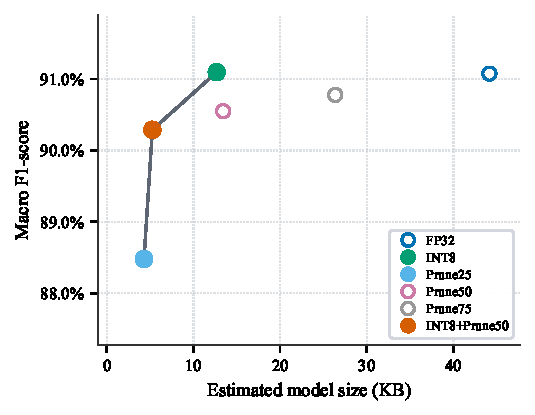
\includegraphics[width=\linewidth]{figures/pareto_front.pdf}
  \caption{Illustrative Pareto front (fold~0, seed~42). Horizontal axis is \emph{estimated} payload,
  not measured TFLite size (Table~\ref{tab:esp32}); k-fold aggregates in
  Table~\ref{tab:kfold-compression}. Frontier: Prune25 $\rightarrow$ INT8+Prune50 $\rightarrow$
  INT8; Prune50/Prune75/FP32 are dominated here. Prune25 \emph{retains} only 25\% of channels
  (most aggressive); Prune75 is mildest.}
  \label{fig:pareto}
\end{figure}

\begin{figure}[!t]
  \centering
  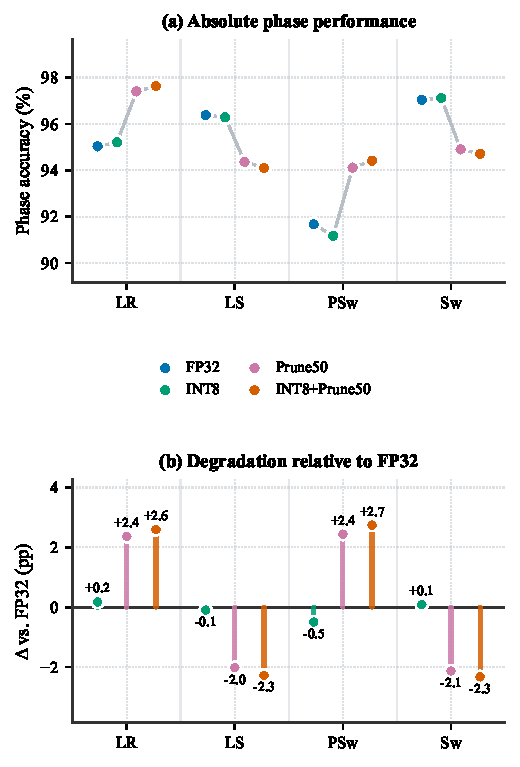
\includegraphics[width=\linewidth]{figures/phase_degradation.pdf}
  \caption{Phase-specific test \emph{accuracy} under compression (fold~0, seed~42).
  Panel~(b) shows that phase \emph{accuracy} can remain nearly flat while phase F1 falls under
  compression (INT8+Prune50: LR accuracy $+0.01$~pp vs.\ LR F1 $-$1.32~pp; PSw F1 $-$1.32~pp).
  Structured pruning also reduces PSw/Sw accuracy (up to $-$1.8~pp), motivating macro and phase F1
  over accuracy alone.}
  \label{fig:phase-degradation}
\end{figure}

\subsection{On-Device Performance on ESP32-C3}
\label{sec:esp32-results}

Table~\ref{tab:esp32} reports on-device latency for five TFLite exports derived from the fold~0,
seed~42 compression checkpoints. Benchmarks replay one fixed normalized $(50,12)$ window in a tight
loop ($N{=}1000$ trials after 20 warmup invocations) without live IMU or BLE I/O.

A non-overlapping 0.5~s window (hop\,=\,window) allows up to 500~ms per inference, but PSw/LR each
span only ${\sim}50$--$100$~ms of the gait cycle, so this cadence cannot resolve a transition
within the window it is detected in. We therefore adopt a clinically motivated \textbf{100~ms}
budget instead: only INT8+Prune50 ($75.7$~ms) meets it; Prune50 ($253$~ms), INT8 ($279.8$~ms),
Prune75 ($510.8$~ms), and FP32 ($856$~ms) do not---the fastest config is also the least accurate
one (Section~\ref{sec:discussion}). The stride-1 (10~ms hop) offline protocol
(Section~\ref{sec:method}) would need sub-10~ms inference, which no config achieves either. FP32
additionally requires a 160~KB tensor arena, reducing minimum free heap to 116~KB vs.\ 156~KB for
the 120~KB-arena configs.

% Measured 2026-07-12 on ESP32-C3 (fold0, seed42; synthetic replay window); Prune75 added 2026-07-23.
\begin{table}[!t]
  \centering
  \caption{On-Device Inference on ESP32-C3 (Standard TCN, fold~0, seed~42)}
  \label{tab:esp32}
  \footnotesize
  \setlength{\tabcolsep}{4pt}
  \renewcommand{\arraystretch}{1.18}
  \begin{tabular*}{\columnwidth}{@{\extracolsep{\fill}} l *{4}{c} @{}}
    \toprule
    \textbf{Config} & \textbf{Mean (ms)} & \textbf{p95 (ms)} & \textbf{TFLite (KB)} & \textbf{Heap (KB)} \\
    \midrule
    FP32            & 856.2 & 856.2 & 52.1 & 116.3 \\
    Prune75         & 510.8 & 510.8 & 34.5 & 156.3 \\
    INT8            & 279.8 & 279.8 & 21.3 & 156.3 \\
    Prune50         & 253.0 & 253.0 & 21.6 & 156.3 \\
    INT8+Prune50    &  75.7 &  75.7 & 13.4 & 156.3 \\
    \bottomrule
  \end{tabular*}

  \vspace{0.2em}
  {\scriptsize
  ESP32-C3 @ 160~MHz; TFLite Micro. Latency/0.5~s window ($N{=}1000$, 20 warmup). Mean and p95
  round to the same value because latency is essentially deterministic on this bare-metal,
  single-core target: max$-$min jitter across all 1000 trials is $<0.08$~ms for every config. Heap
  = min.\ free dynamic heap; arena 120~KB (all but FP32) or 160~KB (FP32); weights in flash. Only
  INT8+Prune50 meets the clinically motivated 100~ms real-time budget (Section~\ref{sec:esp32-results}).}
\end{table}


\section{Discussion}
\label{sec:discussion}

\subsection{Variance Across Folds and Seeds}

Across the $K{=}5$ folds$\times$3 seeds ($N{=}15$) baseline runs, $\sigma_{\mathrm{fold}}{=}1.38$~pp
exceeds $\sigma_{\mathrm{seed}}{=}0.28$~pp for TCN, so performance spread (Table~\ref{tab:baseline})
primarily reflects which subjects appear in each test fold rather than initialization noise.

\subsection{Vulnerability of Transition Phases}

Across k-fold compression (Table~\ref{tab:kfold-compression}), PSw F1 shows the largest
pruning-related degradation relative to FP32 ($-$3.75~pp Prune25, $-$1.59~pp Prune50 5~ep,
$-$1.79~pp INT8+Prune50), while INT8 alone changes it by only $+0.03$~pp ($p{=}0.30$); LR is
equally sensitive ($-$6.98~pp, Prune25), and the fine-tune ablation confirms only partial PSw
recovery. This may be confounded with support/difficulty, since LR/PSw are simultaneously the only
transition phases and lowest-support classes ($\sim$6\%/5\%); still, relative to each phase's own
FP32 F1 under Prune25, LR/PSw lose more ($-$8.1\%, $-$4.5\%) than steady-state LS/Sw ($-$1.3\%,
$-$1.1\%)---not purely a baseline-F1 artifact, though collinear with only four classes. The same
ordering reappears, more mildly, under real deployed compression: LR F1 falls $-$1.6~pp under
plain INT8 and $-$7.6~pp under INT8+Prune50, vs.\ only $-$0.2~pp and $-$0.9~pp for Sw
(Table~\ref{tab:int8-real})---a general, if modest for quantization alone, compression signature.

\subsection{Weight- vs.\ Activation-Quantization Tolerance}

INT8 weight quantization alone preserved macro F1 within 0.01~pp of FP32 ($p{=}0.30$), so TCN's
dilated receptive field and narrow hidden width tolerate 8-bit \emph{weight} precision well. The
real deployed model additionally quantizes \emph{activations}, costing a further
$0.72\pm0.60$~pp---small but statistically significant across all 15 pairs (Table~\ref{tab:int8-real}),
indicating some activation noise compounds across the four dilated blocks that weight quantization
alone does not show. This roughly doubles under INT8+Prune50 ($3.56\pm2.10$~pp), suggesting pruned
channels leave less redundancy to absorb it. Pruning alone removes capacity by a different,
gap-free mechanism (Prune50 0.53~pp below FP32 even at 50-epoch fine-tuning), but PSw suffers under
both.

\textbf{Efficiency-accuracy trade-off:} higher accuracy does not imply faster inference. At a
lenient 500~ms (non-overlapping window) budget, INT8 (real $90.15\%\pm1.35\%$, 279.8~ms) nearly
matches Prune75's accuracy while staying real-time; but PSw/LR's ${\sim}50$--$100$~ms duration
motivates the stricter 100~ms budget (Section~\ref{sec:esp32-results}), which only INT8+Prune50
meets, at a real accuracy cost roughly 5$\times$ plain INT8's. Both the proxy's residual optimism
and any config's on-device latency require empirical confirmation before recommending a deployment
target from PyTorch-side numbers alone.

\subsection{Limitations}

\begin{itemize}
  \item Results derive from a single public dataset (NONAN GaitPrint; generalization untested);
        ESP32-C3 benchmarks used a synthetic replay window (fold~0, seed~42) with no live IMU/BLE.
  \item Test stride~1 yields highly overlapping windows; per-subject blocked aggregation mitigates
        this, but Wilcoxon tests use fold$\times$seed aggregates ($N{=}15$, not fully independent),
        bounding the smallest signed-rank $p$ at $6.10\times10^{-5}$; Holm--Bonferroni correction
        changes no conclusion.
  \item Prune25/75+INT8 combinations were not part of the compression grid (no real-TFLite gap
        measured); power (mW) was not measured; latency used TFLite Micro reference kernels
        (Chirale\_TensorFlowLite).
\end{itemize}

\section{Conclusion}
\label{sec:conclusion}

This study evaluated how INT8 quantization and structured pruning affect phase-specific accuracy
in a Standard TCN for gait phase detection. TCN achieved $90.87\%\pm1.47\%$ macro F1 under
$K{=}5\times3$ cross-validation, the highest mean among compared architectures while remaining
microcontroller-deployable. A PyTorch weight-only QDQ proxy showed INT8 statistically equivalent
to FP32 ($p{=}0.30$); the \emph{actual deployed} full-integer TFLite model, evaluated on the same
$N{=}15$ protocol, confirmed this proxy is reasonable but not exact---a further $0.72\pm0.60$~pp
real cost that roughly doubles under combined INT8+Prune50 ($3.56\pm2.10$~pp), so the
proxy--deployment gap widens as compression techniques stack. Structured pruning incurs
severity-dependent losses (Prune50: $-$1.47~pp; Prune75: $-$0.70~pp, both $p{<}0.001$), partly
recoverable with longer fine-tuning, and PSw/LR remained the most compression-sensitive phases
throughout. Because PSw/LR each span only ${\sim}50$--$100$~ms of the gait cycle, we adopt a
clinically motivated 100~ms real-time budget: only INT8+Prune50 (75.7~ms) meets it, exposing a
genuine tension between the one config fast enough for real-time transitions and the higher, more
reliable accuracy of the slower alternatives. Future work will validate live IMU streaming and
additional cohorts.

% Acknowledgment omitted for double-anonymous review.

\begin{thebibliography}{00}
\footnotesize
\bibitem{ref1} W. Choi and M.-T. Choi, ``Deep learning-based gait phase detection using
shank-mounted IMU data: Classification approach,'' \textit{PLOS ONE}, vol.~21, no.~4, p.~e0344002,
2026, doi: 10.1371/journal.pone.0344002.
\bibitem{ref2} S. Bai, J. Z. Kolter, and V. Koltun, ``An empirical evaluation of generic
convolutional and recurrent networks for sequence modeling,'' \textit{arXiv preprint
arXiv:1803.01271}, 2018.
\bibitem{ref3} B. Jacob et al., ``Quantization and training of neural networks for efficient
integer-arithmetic-only inference,'' in \textit{Proc. IEEE Conf. Computer Vision and Pattern
Recognition (CVPR)}, 2018, pp.~2704--2713.
\bibitem{ref4} S. Han, H. Mao, and W. J. Dally, ``Deep compression: Compressing deep neural
networks with pruning, trained quantization and Huffman coding,'' in \textit{Proc. Int. Conf.
Learning Representations (ICLR)}, 2016.
\bibitem{ref5} R. David et al., ``TensorFlow Lite Micro: Embedded machine learning for TinyML
systems,'' in \textit{Proc. Machine Learning and Systems (MLSys)}, vol.~3, 2021, pp.~800--811.
\bibitem{ref6} Espressif Systems, \textit{ESP32-C3 Technical Reference Manual}, version~1.3, 2024.
\bibitem{ref7} T. M. Wiles et al., ``NONAN GaitPrint: An IMU gait database of healthy young
adults,'' \textit{Scientific Data}, vol.~10, no.~867, 2023, doi: 10.1038/s41597-023-02704-z.
\end{thebibliography}

\end{document}
